\documentclass[10pt]{beamer}
\usepackage{amsmath, graphicx, textcomp,multirow,subfigure}

\usetheme{Rochester}
\usepackage{natbib} 
\usepackage{wrapfig}

\usetheme{PaloAlto}
\setbeamertemplate{footline}{\insertframenumber/\inserttotalframenumber}

\newcommand{\true}{{\mbox{\hspace*{0cm}\tiny{\sf true}} }}
\newcommand{\means}{{\mbox{\hspace*{0cm}\tiny{\sf means}} }}
\newcommand{\logit}{\ensuremath{\mbox{logit}}}

\title{Classifier Technology and the Illusion of Progress}
\author{Elizabeth Sweeney}
\institute{Department of Biostatistics  \\ Johns Hopkins Bloomberg School of Public Health}
\date{January 29, 2015}

\begin{document}

\frame{\titlepage}
	\frametitle{Reference} 

 

\frame{

Hand, David J. "Classifier technology and the illusion of progress." Statistical Science 21.1 (2006): 1-14.

}


\frame{ 
\frametitle{The Classification Task}

\begin{enumerate} 
\item We have random variables $(X,Y)$ such that  $X \in \mathbb{R}^d$ and $Y \in \{0, 1 \}$. 
\item Let $g: \mathbb{R}^d \rightarrow \{0, 1\}$ 
\item The error probability is $P_g \left( X, Y \right) = \mathbb{P}  \{ g (X) \neq Y \}$
\item The classification task is to find $g$ that minimizes $P_g \left( X, Y \right)$
\item The functions g are called ``classifiers"
\end{enumerate} 

}



\frame{ 
\frametitle{The Supervised Classification Task}

\begin{enumerate} 
\item In practice we have a training sequence $\xi_n = \left( (X_1, Y_1), (X_2, Y_2), ... (X_n, Y_n)  \right)$  where $\left(X_k, Y_k \right)$ are assumed to be iid from $\left(X, Y \right) $
\item We then estimate $Y$ from $g_n \left(X, \xi_n \right)$, minimizing $  \mathbb{P}  \{ g_n (X, \xi_n) \neq Y \}$
\end{enumerate} 

}


\frame{ 
\frametitle{Classifiers}

\begin{figure}
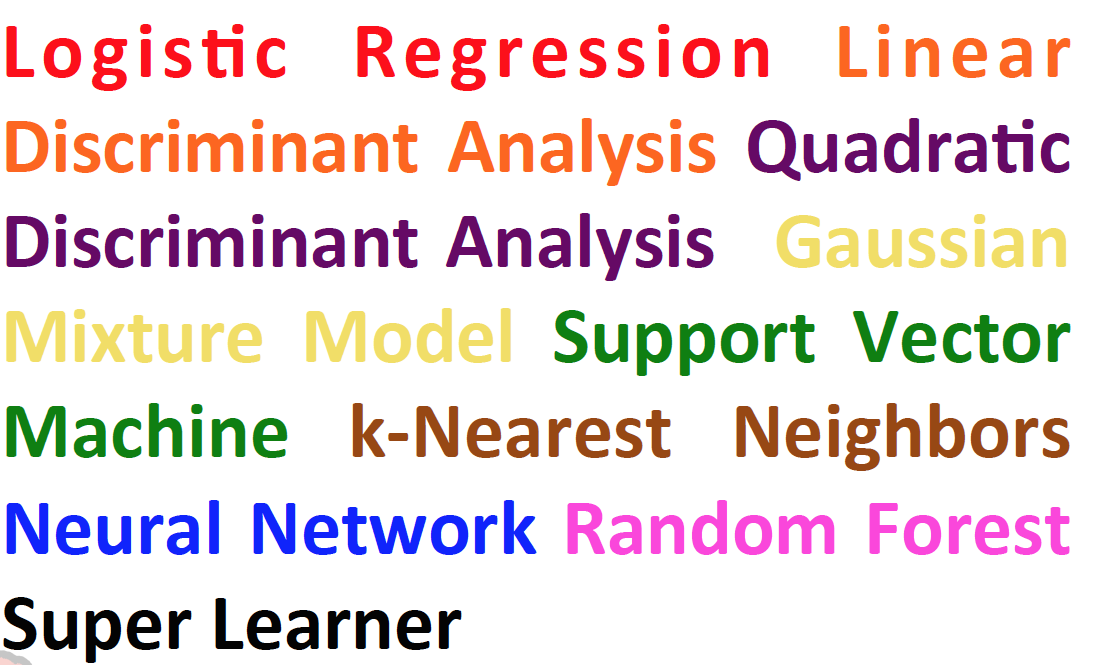
\includegraphics[width=.8 \linewidth]{Classifiers.png}
\end{figure} 

}



\frame{

``A large number of comparative studies have been conducted in attempts to establish the relative superiority of these [classification] methods.   This paper argues that these comparisons often fail to take into account important aspects of real problems, so that apparent superiority of more sophisticated methods may be something of an illusion"  

\bigskip

\citep{hand2006classifier}
}




\frame{
	\frametitle{Outline}

\begin{enumerate}
\item Marginal Improvements 
\item Design Sample Selection
\item Problem Uncertainty 
\item Interpreting Empirical Comparisons 
\end{enumerate} 

}


\frame{
	\frametitle{Marginal Improvements}
\begin{enumerate} 
\item Large gains in predictive accuracy are won using relatively simple models -- potential gains decrease in size as the modeling process is taken further. 
\item Extra accuracy is achieved by modeling ``minor" aspects of the distribution

\end{enumerate} 

}



\frame{
	\frametitle{Marginal Improvements: Linear Regression Example }

A simple regression case, with response variable y and predictors $\mathbf{x} = \left(x_1, ... x_d \right)^{T}$.  The correlation matrix for $\left( \mathbf{x}^{T}, y \right)$ is 

\begin{equation} 
\Sigma = \left[\begin{array}{cc} \Sigma_{11} & \Sigma_{12} \\ \Sigma_{21} &  \Sigma_{22} \end{array}\right] =  \left[\begin{array}{cc} (1 - \rho) \mathbf{I} + \rho \mathbf{11}^{T} & \mathbf {\tau}  \\  \mathbf {\tau}^{T} &  1 \end{array}\right]
\end{equation} 

So the correlation between each pair of predictors is $\rho$ and between each predictor and the response is $\tau$.  We assume $\tau, \rho \geq 0$. 


}

\frame{
	\frametitle{Marginal Improvements: Linear Regression Example }

The conditional variance of $y$ given $\mathbf{x}$ is 

\begin{equation} 
V \left( d \right) = \Sigma_{22} - \Sigma_{21} \Sigma_{11} ^{-1}   \Sigma_{12}
\end{equation} 

as 

\begin{equation} 
\Sigma_{11} ^{-1}   = \frac{1}{1 - \rho} \left \{ \mathbf{I} - \frac{\rho \mathbf{11}^{T}}{1 + \left( d - 1 \right) \rho } \right \} 
\end{equation} 


we have that 

\begin{equation} 
V \left( d \right) = 1 - \frac{d \tau^2}{1 - \rho} + \frac{ \rho d^2 \tau^2}{ \left( 1 + (d - 1) \rho \right) \left( 1 - \rho \right) }
\end{equation} 
}



\frame{
	\frametitle{Marginal Improvements: Linear Regression Example }
Let $X \left( d + 1 \right)$ be the decrease in the conditional variance of $y$ given $\mathbf{x}$ after adding another predictor to the model. 

\begin{align} 
X \left( d + 1 \right) & = V \left( d \right) - V \left( d + 1 \right) \\
& = \frac{\tau^2}{1 - \rho} + \frac{ \rho \tau^2}{1 - \rho} \left[ \frac{d^2}{1 + (d - 1) \rho } - \frac{ (d + 1)^2}{1 + d \rho } \right]
\end{align} 
}

\frame{
	\frametitle{Marginal Improvements: Linear Regression Example }

\begin{equation} 
X \left( d + 1 \right)  = \frac{\tau^2}{1 - \rho} + \frac{ \rho \tau^2}{1 - \rho} \left[ \frac{d^2}{1 + (d - 1) \rho } - \frac{ (d + 1)^2}{1 + d \rho } \right]
\end{equation}

\bigskip 

\textbf{Case \#1}: The predictor variables are uncorrelated, i.e. $\rho = 0$

\begin{equation} 
X \left(d = 1 \right) = \tau^2 
\end{equation} 



 
}


\frame{
	\frametitle{Marginal Improvements: Linear Regression Example }

\textbf{Case \#2}: The predictor variables are correlated, i.e. $\rho > 0$

\begin{figure}
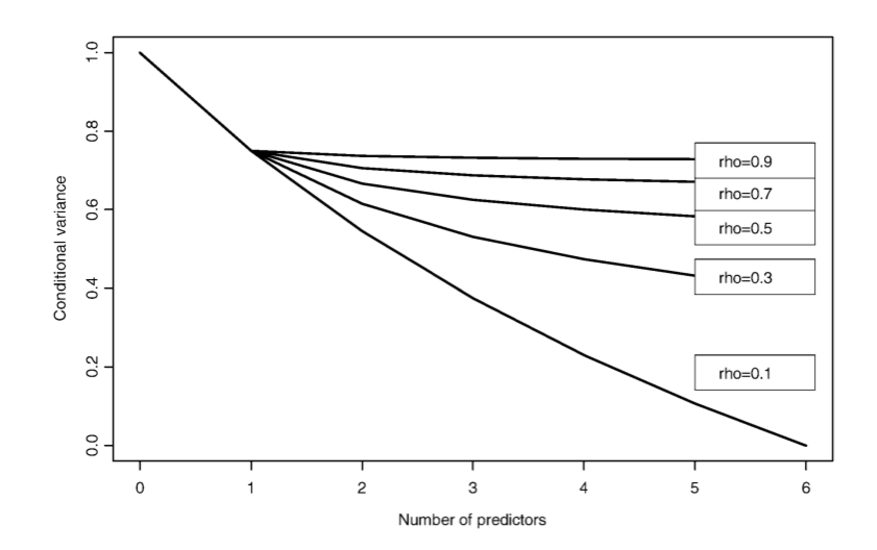
\includegraphics[width=.8 \linewidth]{cond_var.pdf}
\end{figure} 



 
}



\frame{
	\frametitle{Marginal Improvements: Effectiveness of Simple Classifiers}

Comparison of Fisher's Linear Discriminant Analysis (LDA) and the ``best" method in the literature on 10 datasets.  


}

\frame{
	\frametitle{Marginal Improvements: Effectiveness of Simple Classifiers}

Fisher's Linear Discriminant Analysis \citep{hastie2009elements} 

\begin{figure}
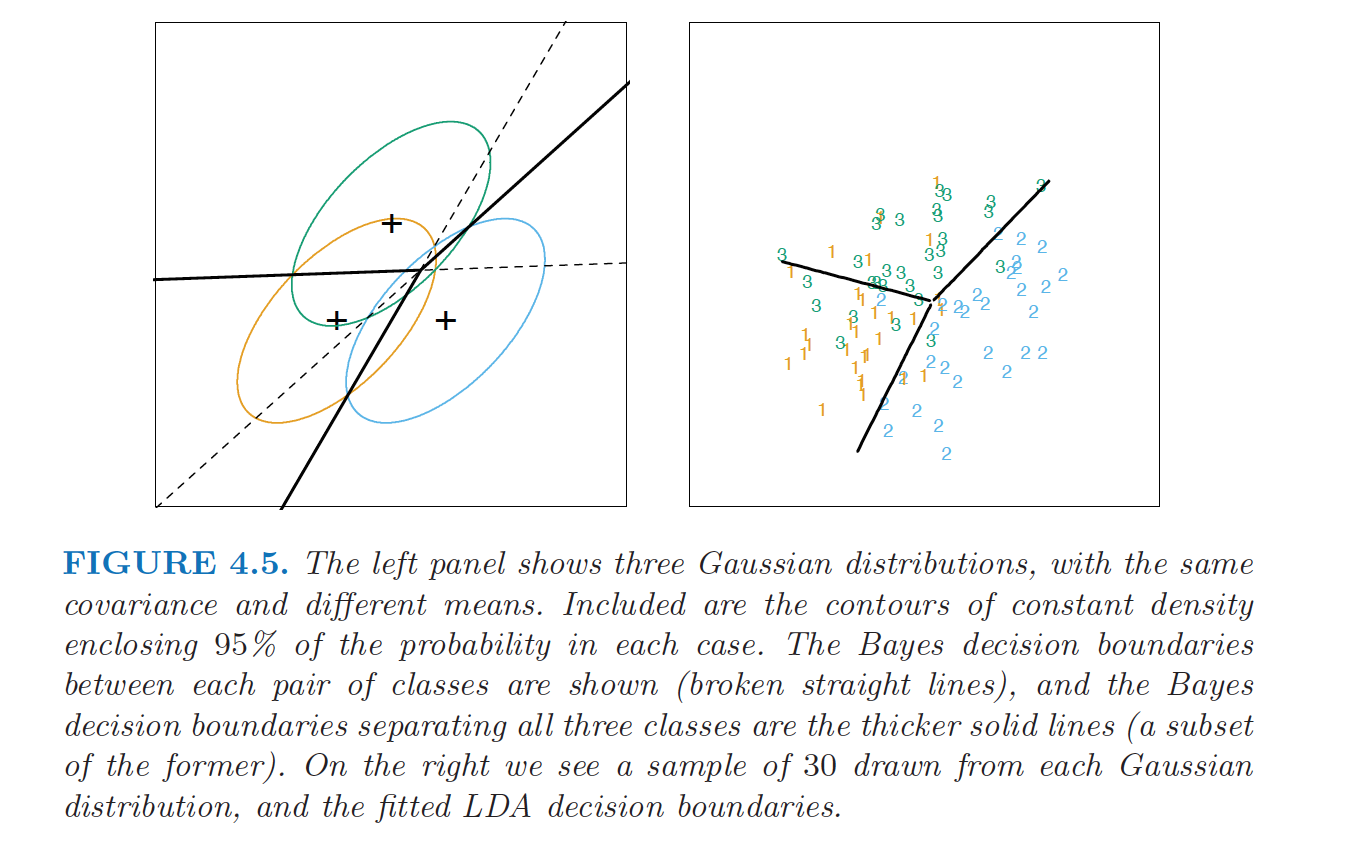
\includegraphics[width=.8 \linewidth]{LDA.png}
\end{figure} 


}


\frame{
	\frametitle{Marginal Improvements: Effectiveness of Simple Classifiers}

\begin{enumerate} 
\item Best method misclassification rate ($m_T$)
\item LDA misclassification rate ($m_L$) 
\item Default rate ($m_0$) -- classify all points to the class with the highest prior probability 
\item Prop linear 
\begin{equation} 
\frac{ m_0 - m_L }{ m_0 - m_T} 
\end{equation} 
\end{enumerate} 

}


\frame{
	\frametitle{Marginal Improvements: Effectiveness of Simple Classifiers}

\begin{figure}
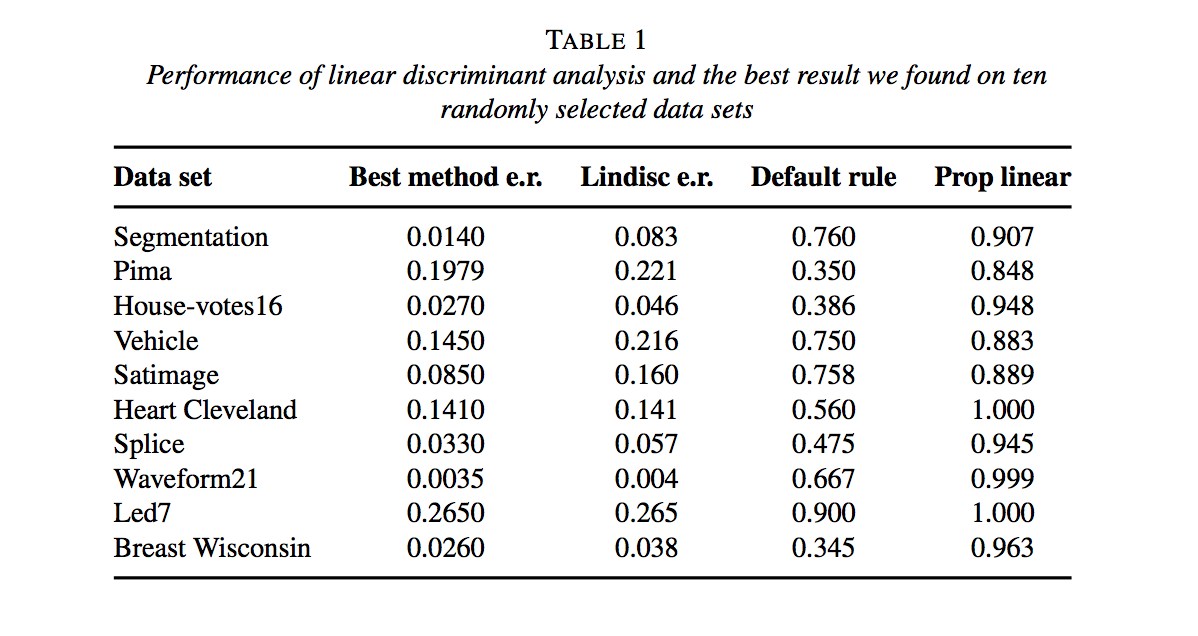
\includegraphics[width=.9 \linewidth]{simple_classifiers_table.png}
\end{figure} 


}


\frame{
	\frametitle{Marginal Improvements: Neural Networks}

\begin{figure}
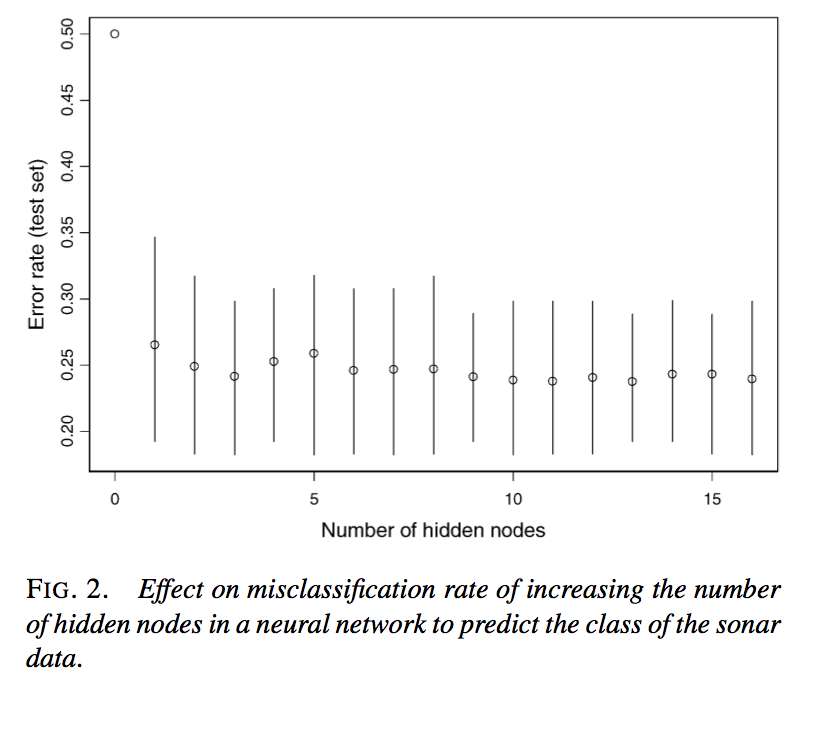
\includegraphics[width=.7 \linewidth]{neural_net.png}
\end{figure} 


}


\frame{
	\frametitle{Design Sample Selection}

\begin{enumerate}
\item In classification, we make the assumption that the data in the design set are randomly drawn from the same distribution as those to be classified in the future. 
\item Issue arise with \textbf{population drift} and \textbf{sample selectivity bias}. 
\end{enumerate} 

}

\frame{
	\frametitle{Design Sample Selection: Population Drift}

\begin{enumerate} 
\item Population distributions are non-stationary. 
\item We make the assumption that our test sample is the same as the sample to be encountered in the future. 
\item Caution against putting too much weight in a classifier on one variable, as the relationship may change over time. 
\end{enumerate} 

}





\frame{
	\frametitle{Design Sample Selection: Population Drift Example 1}

The validation data consists of labels ``good" and ``bad" and the value of 17 predictor variables for 92,258 customers taking our unsecured personal loans with 24-month term given by a major UK bank during the period of January 1st 1993 to November 30th 1997, with 8.86\% of customers belonging to the ``bad" class.

\bigskip

The model is trained on data just preceding this time period. 


}



\frame{
	\frametitle{Design Sample Selection: Population Drift Example 1}

\begin{figure}
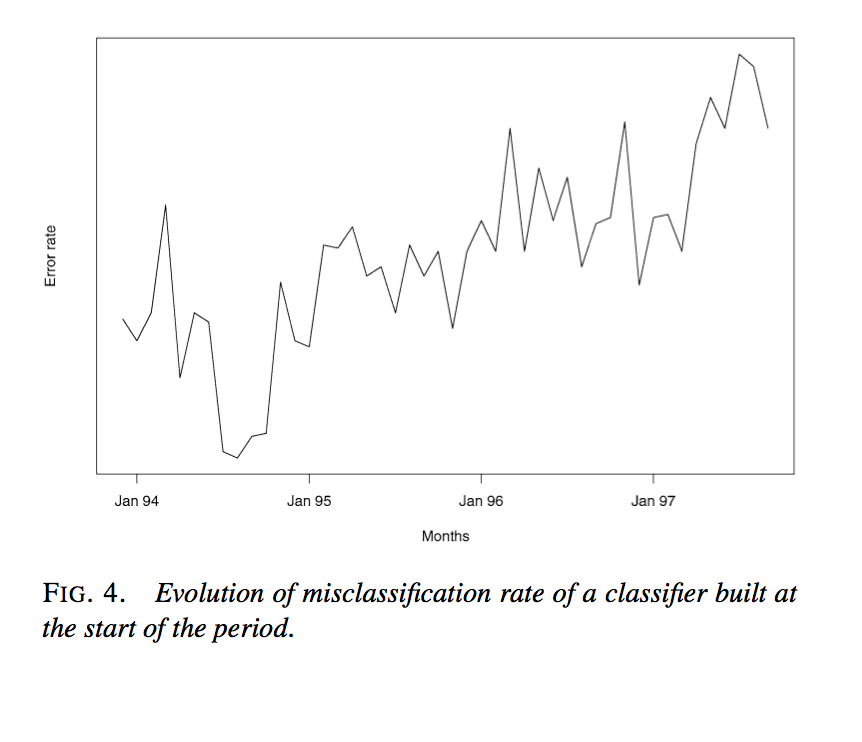
\includegraphics[width=.7 \linewidth]{drift1.png}
\end{figure} 


}

\frame{
	\frametitle{Design Sample Selection: Population Drift Example 2}

A set of $60,000$ customers.

\bigskip 

For the design set  customers $1, 3, 5, 7, . . . , 4999$ were used. 

\bigskip 

The the classifier is applied to alternate customers, beginning with the second,
up to the $60,000^{th}$ customer. ( i.e. different
customers were used for designing and testing) 


}



\frame{
	\frametitle{Design Sample Selection: Population Drift Example 2}

\begin{figure}
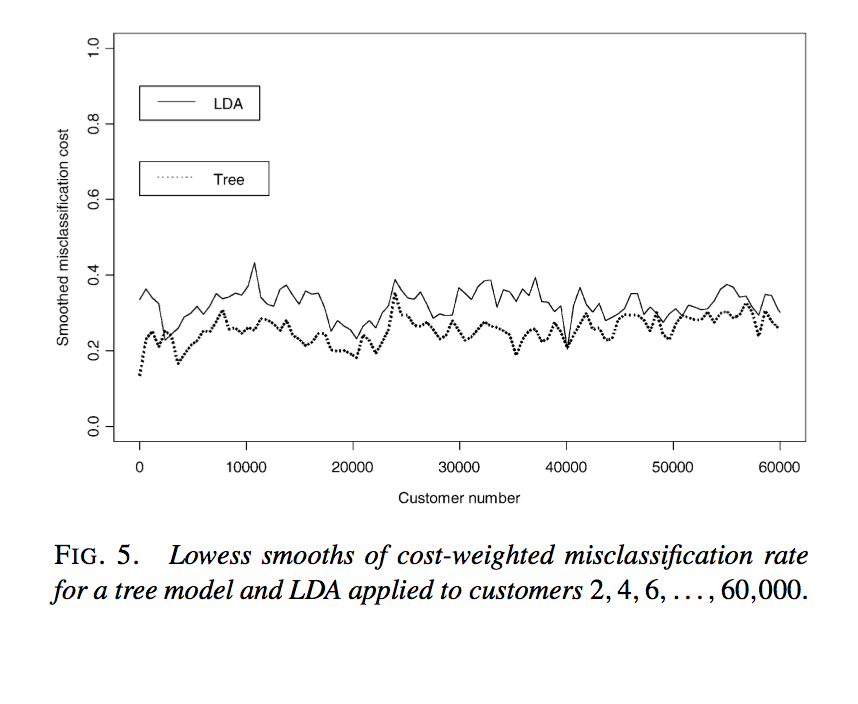
\includegraphics[width=.7 \linewidth]{drift2.png}
\end{figure} 


}

\frame{
	\frametitle{Design Sample Selection: Sample Selectivity Bias}

\begin{enumerate} 
\item Why should we model the subtler aspects of the distributions if the design sample is drawn from a distribution distorted in some way from the original sample
\item Example: Data sampled from one hospital, model to be generalized to other hospitals 
\end{enumerate} 
}


\frame{
	\frametitle{Problem Uncertainty }
Other ways in which classification can go awry....
\begin{enumerate} 
\item Error in Class Labels
\item Arbitrariness in the Class Definition 
\item Optimization Criteria and Performance Assessment 
\end{enumerate} 

}

\frame{
	\frametitle{Problem Uncertainty: Error in Class Labels}
Assumption of classical supervised classification paradigm is that there are no errors in the class labels.  Let $p \left( 1 | \mathbf{x} \right)$ and $p \left( 2 | \mathbf{x} \right)$ be the true posterior class probabilities.  Let $\delta$ be the small proportion of each class incorrectly believed to come from the other class.  Let $p^*(1| \mathbf{x})$ denote our apparent posterior probability for class 1.  Then we will have 

\begin{equation}
p^*(1| \mathbf{x}) = ( 1 - \delta ) p \left( 1 | \mathbf{x} \right) + \delta p \left( 2 | \mathbf{x} \right)
\end{equation} 
}


\frame{
	\frametitle{Problem Uncertainty: Error in Class Labels}
Let $r(x)$ be the true odds ratio

\begin{equation} 
r \left( x \right) = \frac{p \left( 1 | \mathbf{x} \right) }{  p \left( 2 | \mathbf{x} \right)}
\end{equation} 

then our apparent odds ratio is 

\begin{align} 
r^* \left( x \right) &=  \frac{p^* \left( 1 | \mathbf{x} \right) }{  p^* \left( 2 | \mathbf{x} \right)} \\
& = \frac{ r \left( \mathbf{x} \right) + \epsilon }{ \epsilon  r \left( \mathbf{x} \right)  + 1 } 
\end{align} 

with $\epsilon = \frac{\delta}{1 - \delta}$
}



\frame{
	\frametitle{Problem Uncertainty: Error in Class Labels}
Let the true optimal decision surface be $r \left( x \right) = k$.   Then the optimal decision surface when errors are present will be  $r^* \left( x \right) = k^*$, then $k^* =  \frac{ ( k + \epsilon ) }{ ( \epsilon k + 1 ) }$.  In the case of equal misclassification costs $k = k^* = 1$, so this does not matter.  But, when classification costs are not equal this will impact your classification. 
}




\frame{
	\frametitle{Problem Uncertainty: Arbitrariness in Class Definition  }
Assumption of supervised classification is that the classes are well defined -- which may not always be true (especially when defining the classes by thresholding a continuous variable) 

\begin{enumerate} 
\item Consumer credit: definition of a person who "defaults" 
\end{enumerate} 

}



\frame{
	\frametitle{Problem Uncertainty: Optimization Criteria and Performance Assessment  }

The difference between the (1) criterion used to choose the model (2) the criterion used to evaluate its performance and (3) the criterion which actually matters in real applications. 

}




\frame{
	\frametitle{Interpreting Empirical Comparisons }

\begin{enumerate} 
\item Different categories of users may be expected to obtain different rankings of classification methods in different studies
\item People may have a ``favorite classifier" 
\item Classification methods may do well on a dataset just by chance 
\end{enumerate} 
}


\frame{
	\frametitle{Interpreting Empirical Comparisons: Ping-Pong Theorem }

``If we reveal to Professor Breiman the performance of our best model and gave him our data, then he could develop an algorithmic random forest, which would outperform our model.  But, if he reveals to us the performance of his model, then we could develop a segmented scorecard which would outperform his model"

\bigskip 

-- Hoadley 

}


\frame{
	\frametitle{References}

 \bibliography{mybib}
\bibliographystyle{apalike}


} 




\end{document}